
\section{Utstyr}
\subsection{Gand RIO-trainer}

Kortet kobles til PLS med en USB kabel og en trenger en USB til seriel
driver (CH340). 

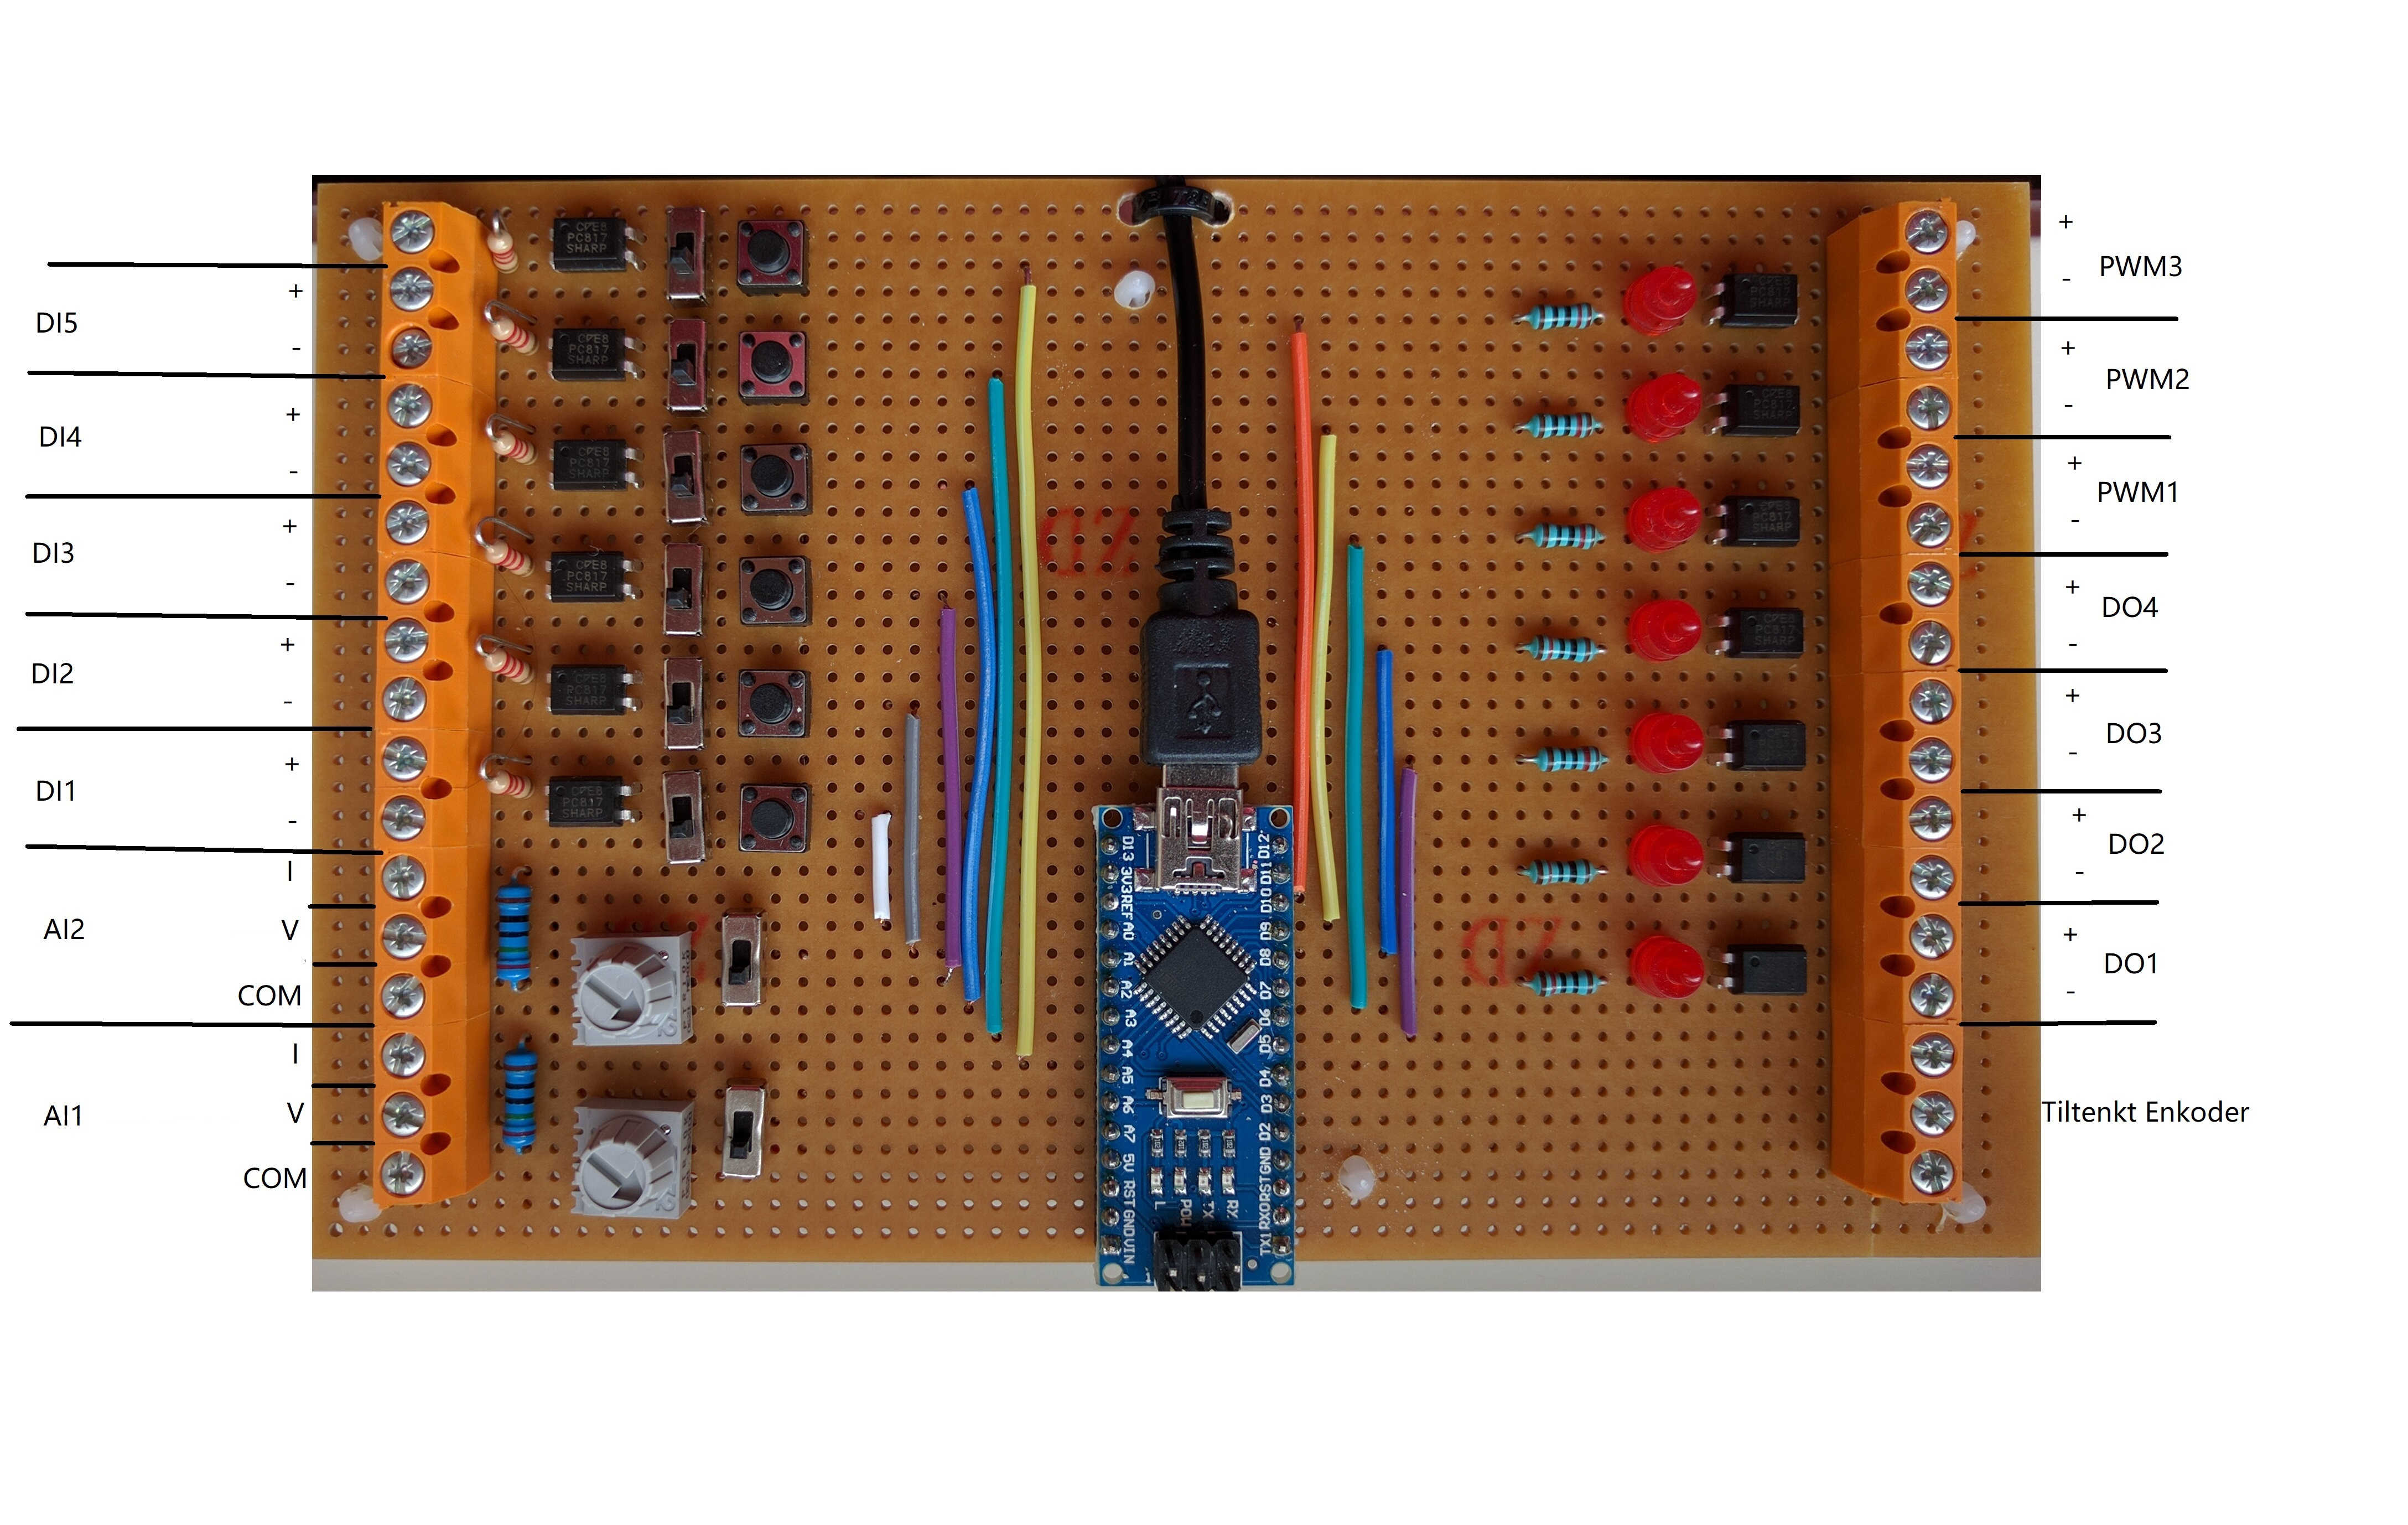
\includegraphics[width=1\textwidth]{./GandRioTrainer.jpg}
\small
\begin{tabular}{|c|c|c|c|}
\hline 
\multicolumn{4}{|c|}{Modbus Data Table}\tabularnewline
\hline 
\hline 
IO & Tilkobling & Register & \tabularnewline
\hline 
Encoder &  & 0000H & Enkoder telleverdi\tabularnewline
\hline 
DO1 & åpen kollektor & 0001H & bit0\tabularnewline
\hline 
DO2 & åpen kollektor & 0001H & bit1\tabularnewline
\hline 
DO3 & åpen kollektor & 0001H & bit2\tabularnewline
\hline 
DO4 & åpen kollektor & 0001H & bit3\tabularnewline
\hline 
PWM1 & åpen kollektor & 0002H & AO 0 (PWM)\tabularnewline
\hline 
PWM2 & åpen kollektor & 0003H & AO 1 (PWM)\tabularnewline
\hline 
PWM3 & åpen kollektor & 0004H & AO 2 (PWM)\tabularnewline
\hline 
DI1 & 24VDC & 0005H & bit0\tabularnewline
\hline 
DI2 & 24VDC & 0005H & bit1\tabularnewline
\hline 
DI3 & 24VDC & 0005H & bit2\tabularnewline
\hline 
DI4 & 24VDC & 0005H & bit3\tabularnewline
\hline 
DI5 & 24VDC & 0005H & bit4\tabularnewline
\hline 
DI6 & 24VDC & 0005H & bit5\tabularnewline
\hline 
AI2 & 4-24mA/0-5V & 0006H & AI2\tabularnewline
\hline 
AI1 & 4-24mA/0-5V & 0007H & AI1\tabularnewline
\hline 
\end{tabular}
\normalsize
\vfil \eject
\subsection{Wago PFC200 på stasjon 3}

Stasjon 3 \\
IP 192.168.0.3\\
web grensesnitt innlogging:\\
user:admin\\
pass:wago\\
\\\\
Codesys innlogging:\\
user:Elev3AUA\\
pass:3AUAGand\\
\section{Instrumenter}
\subsection{multimeter}
\subsection{loop claibrator}
\subsection{nettverkstester}
\subsection{megger}
\subsection{kontinuitetstester}





